\documentclass[openany]{book}

\usepackage[margin=1in]{geometry}
\usepackage{amsmath,amsfonts,amsthm, amssymb}
\usepackage{yhmath}
\usepackage{mathrsfs}
\usepackage{mathtools}
\usepackage{xcolor}
\usepackage{graphicx}
\usepackage{comment}
\usepackage{tikz-cd}
\usepackage{quiver}
\renewcommand{\familydefault}{ppl}
\newcommand{\tr}{\text{tr}}
\newcommand{\R}{\mathbb{R}}
\newcommand{\E}{\mathbb{E}}
\newcommand{\Z}{\mathbb{Z}}
\newcommand{\C}{\mathbb{C}}
\newcommand{\F}{\mathbb{F}}
\newcommand{\la}{\langle}
\newcommand{\ra}{\rangle}
\newcommand{\colim}{\text{colim}}
\DeclareMathOperator{\im}{im}
\let\oldemptyset\emptyset
\let\emptyset\varnothing
\newcommand{\tor}{\text{Tor}}
\newcommand{\id}{\text{id}}
\newcommand{\ext}{\text{Ext}}
\newcommand{\ptop}{\text{PTop}}
\newcommand{\pt}{\text{pt}}
\newcommand{\ach}{\text{Ach}}
\newcommand{\Q}{\mathbb{Q}}
\newcommand{\gal}{\text{Gal}}


\usepackage{thmtools,thm-restate}

% Fixing mdframed skip below
% See https://tex.stackexchange.com/a/292090/143086
\usepackage[framemethod=TikZ]{mdframed}
\usepackage{xpatch}
\makeatletter
\xpatchcmd{\endmdframed}
	{\aftergroup\endmdf@trivlist\color@endgroup}
	{\endmdf@trivlist\color@endgroup\@doendpe}
	{}{}
\makeatother

\definecolor{huilightpink}{HTML}{fff2fe}
\definecolor{huidarkpink}{HTML}{d955b7}
\declaretheoremstyle[
	mdframed={
		backgroundcolor=huilightpink,
		linecolor=huidarkpink,
		rightline=false,
		topline=false,
		bottomline=false,
		linewidth=2pt,
		innertopmargin=5pt,
		innerbottommargin=8pt,
		innerleftmargin=8pt,
		leftmargin=-2pt,
		skipbelow=2pt,
		nobreak
	},
	headfont=\normalfont\bfseries\color{huidarkpink}
]{huipinkbox}
\declaretheorem[style=huipinkbox,name=Theorem,within=chapter]{thm}
\declaretheorem[style=huipinkbox,name=Theorem,sibling=thm]{theorem}




\begin{comment}
\definecolor{huilightyellow}{HTML}{fff5d6}
\definecolor{huidarkyellow}{HTML}{fcad03}
\declaretheoremstyle[
	mdframed={
		backgroundcolor=huilightyellow,
		linecolor=huidarkyellow,
		rightline=false,
		topline=false,
		bottomline=false,
		linewidth=2pt,
		innertopmargin=5pt,
		innerbottommargin=8pt,
		innerleftmargin=8pt,
		leftmargin=-2pt,
		skipbelow=2pt,
		nobreak
	},
	headfont=\normalfont\bfseries\color{huidarkyellow}
]{huiyellowbox}
\declaretheorem[style=huiyellowbox,name=Proposition,within=chapter]{prop}
\end{comment}



\definecolor{huilightpurple}{HTML}{faf2ff}
\definecolor{huidarkpurple}{HTML}{912ed9}
\declaretheoremstyle[
	mdframed={
		backgroundcolor=huilightpurple,
		linecolor=huidarkpurple,
		rightline=false,
		topline=false,
		bottomline=false,
		linewidth=2pt,
		innertopmargin=5pt,
		innerbottommargin=8pt,
		innerleftmargin=8pt,
		leftmargin=-2pt,
		skipbelow=2pt,
		nobreak
	},
	headfont=\normalfont\bfseries\color{huidarkpurple}
]{huipurplebox}
\declaretheorem[style=huipurplebox,name=Proposition,within=chapter]{prop}



% \definecolor{huilightpurple}{HTML}{faf2ff}
% \definecolor{huidarkpurple}{HTML}{912ed9}
% \declaretheoremstyle[
% 	mdframed={
% 		backgroundcolor=huilightpurple,
% 		linecolor=huidarkpurple,
% 		rightline=false,
% 		topline=false,
% 		bottomline=false,
% 		linewidth=2pt,
% 		innertopmargin=5pt,
% 		innerbottommargin=8pt,
% 		innerleftmargin=8pt,
% 		leftmargin=-2pt,
% 		skipbelow=2pt,
% 		nobreak
% 	},
% 	headfont=\normalfont\bfseries\color{huidarkpurple}
% ]{huipurplebox}
\declaretheorem[style=huipurplebox,name=Lemma,within=chapter]{lem}


\definecolor{lightpink}{HTML}{f0f6fc}
\definecolor{darkpink}{HTML}{2c72b8}
\declaretheoremstyle[
	mdframed={
		backgroundcolor=lightpink,
		linecolor=darkpink,
		rightline=false,
		topline=false,
		bottomline=false,
		linewidth=2pt,
		innertopmargin=5pt,
		innerbottommargin=8pt,
		innerleftmargin=8pt,
		leftmargin=-2pt,
		skipbelow=2pt,
		nobreak
	},
	headfont=\normalfont\bfseries\color{darkpink}
]{pinkbox}
\declaretheorem[style=pinkbox,name=Definition,within=chapter]{defn}


\definecolor{huilightblue}{HTML}{edf9ff}
\definecolor{huidarkblue}{HTML}{4b79db}
\declaretheoremstyle[
	mdframed={
		backgroundcolor=huilightblue,
		linecolor=huidarkblue,
		rightline=false,
		topline=false,
		bottomline=false,
		linewidth=2pt,
		innertopmargin=5pt,
		innerbottommargin=8pt,
		innerleftmargin=8pt,
		leftmargin=-2pt,
		skipbelow=2pt,
		nobreak
	},
	headfont=\normalfont\bfseries\color{huidarkblue}
]{huiblueblox}
\declaretheorem[style=huiblueblox,name=Example,within=chapter]{example}



% \definecolor{huilightblue}{HTML}{edf9ff}
% \definecolor{huidarkblue}{HTML}{4b79db}
% \declaretheoremstyle[
% 	mdframed={
% 		backgroundcolor=huilightblue,
% 		linecolor=huidarkblue,
% 		rightline=false,
% 		topline=false,
% 		bottomline=false,
% 		linewidth=2pt,
% 		innertopmargin=5pt,
% 		innerbottommargin=8pt,
% 		innerleftmargin=8pt,
% 		leftmargin=-2pt,
% 		skipbelow=2pt,
% 		nobreak
% 	},
% 	headfont=\normalfont\bfseries\color{huidarkblue}
% ]{huiblueblox}
% \declaretheorem[style=huiblueblox,name=Example,within=chapter]{example}

% \declaretheoremstyle[
% 	mdframed={
% 		backgroundcolor=huilightblue,
% 		linecolor=huidarkblue,
% 		rightline=false,
% 		topline=false,
% 		bottomline=false,
% 		linewidth=2pt,
% 		innertopmargin=5pt,
% 		innerbottommargin=8pt,
% 		innerleftmargin=8pt,
% 		leftmargin=-2pt,
% 		skipbelow=2pt,
% 		nobreak
% 	},
% 	headfont=\normalfont\bfseries\color{huidarkblue}
% ]{huiblueblox}
\declaretheorem[style=huiblueblox,name=Problem,within=chapter]{prob}



% \declaretheoremstyle[
% 	mdframed={
% 		backgroundcolor=huilightblue,
% 		linecolor=huidarkblue,
% 		rightline=false,
% 		topline=false,
% 		bottomline=false,
% 		linewidth=2pt,
% 		innertopmargin=5pt,
% 		innerbottommargin=8pt,
% 		innerleftmargin=8pt,
% 		leftmargin=-2pt,
% 		skipbelow=2pt,
% 		nobreak
% 	},
% 	headfont=\normalfont\bfseries\color{huidarkblue}
% ]{huiblueblox}
\declaretheorem[style=huiblueblox,name=Exercise,within=chapter]{exer}
\declaretheorem[style=huipinkbox, name=Corollary, within=chapter]{cor}





















\newcommand{\nirwarnsymbol}{%
	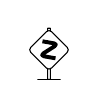
\begin{tikzpicture}[baseline=(x.base)]
		\draw[rounded corners=.01em] (-.05em,-1.07em)rectangle(.05em,.78em);
		\draw[fill=white,rounded corners=1.3] (0,.75em)--(.75em,0)--(0,-.75em)--(-.75em,0)--cycle;
		\draw[line width=0.2mm, line cap=round](-.4em,-1.07em)--(.4em,-1.07em);
		\node(x) at (0,0em) {};
		% Thank you https://tex.stackexchange.com/a/262510
		\draw[
			line cap=but,
			line join=round,
			x=.5em,
			line width=0.5mm,
			y=1*(height("Z")-\pgflinewidth)*(1-sin(10)),
			rotate=-10,
			rounded corners=1.5pt,
		](-0.57, 0.57) -- (0.57, 0.57) -- (-0.57, -0.57) -- (0.57, -0.57);
	\end{tikzpicture}%
}

%%%%%%%%%%%%%%%%%%%%%%%%%%%%%%%%%%%%%%%%%%%% MARGINS
\usepackage{marginnote}
% Thank you https://tex.stackexchange.com/a/472882
% Makes marginnotes always appear on the left, apparently
%
\makeatletter
\long\def\@mn@@@marginnote[#1]#2[#3]{%
	\begingroup
		\ifmmode\mn@strut\let\@tempa\mn@vadjust\else
			\if@inlabel\leavevmode\fi
			\ifhmode\mn@strut\let\@tempa\mn@vadjust\else\let\@tempa\mn@vlap\fi
		\fi
		\@tempa{%
			\vbox to\z@{%
				\vss
				\@mn@margintest
				\if@reversemargin\if@tempswa
						\@tempswafalse
					\else
						\@tempswatrue
				\fi\fi

					\llap{%
						\vbox to\z@{\kern\marginnotevadjust\kern #3
							\vbox to\z@{%
								\hsize\marginparwidth
								\linewidth\hsize
								\kern-\parskip
								%\mn@parboxrestore
								\marginfont\raggedleftmarginnote\strut\hspace{\z@}%
								\ignorespaces#1\endgraf
								\vss
							}%
							\vss
						}%
						\if@mn@verbose
							\PackageInfo{marginnote}{xpos seems to be \@mn@currxpos}%
						\fi
						\begingroup
							\ifx\@mn@currxpos\relax\else\ifx\@mn@currpos\@empty\else
									\kern\@mn@currxpos
							\fi\fi
							\ifx\@mn@currpage\relax
								\let\@mn@currpage\@ne
							\fi
							\if@twoside\ifodd\@mn@currpage\relax
									\kern-\oddsidemargin
								\else
									\kern-\evensidemargin
								\fi
							\else
								\kern-\oddsidemargin
							\fi
							\kern-1in
						\endgroup
						\kern\marginparsep
					}%
			}%
		}%
	\endgroup
}
\makeatother
%
% Mostly for todonotes
\renewcommand{\marginpar}{\marginnote}
%%%%%%%%%%%%%%%%%%%%%%%%%%%%%%%%%%%%%%%%%%%% /MARGINS

\definecolor{nirlightred}{RGB}{250, 220, 220}
\definecolor{nirdarkred}{HTML}{f40000}
\declaretheoremstyle[
	mdframed={
		backgroundcolor=nirlightred,
		linecolor=nirdarkred,
		rightline=false,
		topline=false,
		bottomline=false,
		linewidth=2pt,
		innertopmargin=5pt,
		innerbottommargin=8pt,
		innerleftmargin=8pt,
		leftmargin=-2pt,
		skipbelow=2pt,
		nobreak
	},
	headfont=\normalfont\bfseries\color{nirdarkred}
]{nirredbox}

% \makeatletter
% \declaretheorem[
% 	style=nirredbox,
% 	name=Warning,
% 	sibling=thm,
% 	% without \leavevmode, the first item in a list gets misformatted
% 	postheadhook={\leavevmode\marginnote{\nirwarnsymbol}[-3pt]%
% 	\ifthmt@thisistheone% restatable makes alignment weird
% 		\hspace{-2.2pt}%
% 	\fi}
% ]{warn}
% \makeatother

\newcommand{\nirideasymbol}{%
	
\begin{tikzpicture}[baseline=(x.base)]
		\draw[rounded corners=.01em] (-.05em,-1.07em)rectangle(.05em,.78em);
		\draw[fill=white,rounded corners=1.3] (0,.75em)--(.75em,0)--(0,-.75em)--(-.75em,0)--cycle;
		\draw[line width=0.2mm, line cap=round](-.4em,-1.07em)--(.4em,-1.07em);
		\node(x) at (0,0em) {};
		\node at (0,0em) {{\textbf{!}}};
	\end{tikzpicture}%
}
\renewcommand{\nirwarnsymbol}{%
	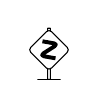
\begin{tikzpicture}[baseline=(x.base)]
		\draw[rounded corners=.01em] (-.05em,-1.07em)rectangle(.05em,.78em);
		\draw[fill=white,rounded corners=1.3] (0,.75em)--(.75em,0)--(0,-.75em)--(-.75em,0)--cycle;
		\draw[line width=0.2mm, line cap=round](-.4em,-1.07em)--(.4em,-1.07em);
		\node(x) at (0,0em) {};
		% Thank you https://tex.stackexchange.com/a/262510
		\draw[
			line cap=but,
			line join=round,
			x=.5em,
			line width=0.5mm,
			y=1*(height("Z")-\pgflinewidth)*(1-sin(10)),
			rotate=-10,
			rounded corners=1.5pt,
		](-0.57, 0.57) -- (0.57, 0.57) -- (-0.57, -0.57) -- (0.57, -0.57);
	\end{tikzpicture}%
}
\makeatletter
\declaretheorem[
	style=nirredbox,
	name=Idea,
	sibling=thm,
	% without \leavevmode, the first item in a list gets misformatted
	postheadhook={\leavevmode\marginnote{\nirideasymbol}[-3pt]%
	\ifthmt@thisistheone% restatable makes alignment weird
		\hspace{-2.2pt}%
	\fi}
]{idea}

\declaretheorem[
	style=nirredbox,
	name=Warning,
	sibling=thm,
	% without \leavevmode, the first item in a list gets misformatted
	postheadhook={\leavevmode\marginnote{\nirwarnsymbol}[-3pt]%
	\ifthmt@thisistheone% restatable makes alignment weird
		\hspace{-2.2pt}%
	\fi}
]{warn}
\makeatother

\title{Algebra Definition Theorem List}

\date{\today}
\author{Hui Sun}


\begin{document}

\maketitle

\tableofcontents
\newpage



\chapter{Category Theory}
\begin{defn}[initial, final]
    Let $\mathcal{C}$ be a category, then object $I$ is initial if for every object $A$, there exists a unique morphism $I\to A$. We say $F$ is final if for every $A$, there exists a unique morphism $A\to F$.
\end{defn}


% \begin{defn}[products and coproducts]
%     Let \( A, B \) be sets, and consider the product \( A \times B \), with the two natural projections:

% \[ A \times B \xrightarrow{\pi_A} A \]

% Then for every set \( Z \) and morphisms

% % \[
% % \begin{tikzcd}
% %  & f_A \arrow[dashrightarrow]{d} & A \\
% % Z & & \\
% %  & f_B \arrow[dashrightarrow]{d} & B
% % \end{tikzcd}
% % \]


% there exists a unique morphism \(\sigma : Z \to A \times B\) such that the diagram

% \[
% \begin{tikzcd}
%  & f_A \arrow[dashrightarrow]{dd} & A \\
% Z \arrow{r}{\sigma} & A \times B \arrow{ur}{\pi_A} \arrow{dr}[swap]{\pi_B} & \\
%  & f_B \arrow[dashrightarrow]{uu} & B
% \end{tikzcd}
% \]

% commutes.

% In this situation, \(\sigma\) is usually denoted \( f_A \times f_B \).
% \end{defn}


% \begin{defn}[coproduct]
%     Let \( A, B \) be objects of a category \( \mathcal{C} \). A coproduct \( A \amalg B \) of \( A \) and \( B \) will be an object of \( \mathcal{C} \), endowed with two morphisms \( i_A : A \to A \amalg B \), \( i_B : B \to A \amalg B \) and satisfying the following universal property: for all objects \( Z \) and morphisms

% \[
% \begin{tikzcd}
% A \arrow{r}{i_A} \arrow[swap]{dr}{f_A} & A \amalg B \arrow[dashed]{d}{\exists! \sigma} & B \arrow{l}[swap]{i_B} \arrow{dl}{f_B} \\
%  & Z & 
% \end{tikzcd}
% \]

% there exists a unique morphism \( \sigma : A \amalg B \to Z \) such that the diagram commutes.

% \end{defn}





\chapter{Group Theory I}
This corresponds to Aluffi Chapter II.

\begin{prop}
    Let $G$ be a group, for all $a,g,h\in G$, if 
    \begin{equation*}
        ga=ha
    \end{equation*}
    then $g=h$.
\end{prop}

\begin{prop}
    Let $g\in G$ have order $n$, then 
    \begin{equation*}
        n\mid |G|
    \end{equation*}
\end{prop}

\begin{cor}
    If $g$ is an element of finite order, and let $N\in\mathbb{Z}$, then 
    \begin{equation*}
        g^N=e \iff N \text{ is a multiple of }|g|
    \end{equation*}
\end{cor}

\begin{prop}
    Let $g\in G$ be of finite order, then $g^m$ also has finite order, for all $m\geq 0$, and 
    \begin{equation*}
        \left|g^m\right|=\frac{\text{lcm}(m,|g|)}{m}=\frac{|g|}{\gcd(m,|g|)}
    \end{equation*}
\end{prop}

\begin{prop}
    If $gh=hg$, then $|gh|$ divides $\text{lcm}(|g|,|h|)$.
\end{prop}


\begin{defn}[Dihedral Group]
    Let $D_{2n}$ denote the group of symmetries of a $n$-sided polynomial, consisting of $n$ rotations and $n$ reflections about lines trhough the origin and a vertex or a midpoint of a side.
\end{defn}

\begin{prop}
    Let $m\in\Z/n\Z$, then 
    \begin{equation*}
        |m|=\frac{n}{\gcd(n,m)}
    \end{equation*} 
\end{prop}

\begin{cor}
    The element $m\in\Z/n\Z$ generates $\Z/n\Z$ if and only if $\gcd(m,n)=1$.
\end{cor}


\begin{defn}[Multiplicative $(\Z/n\Z)^\times$]
    The multiplicative group of $\Z/n\Z$ is 
    \begin{equation*}
        \left(\Z/n\Z\right)^\times=\left\{m\in\Z/n\Z: \gcd(m,n)=1\right\}
    \end{equation*}
\end{defn}

\begin{prop}
    Let $\varphi:G\to H$ be a homomorphism, and let $g\in G$ be an element of finite order, then $|\varphi(g)|$ divides $|g|$.

    For example, there is no nontrivial homomorphism from $\Z/n\Z$ to $\Z$.
\end{prop}

\begin{prop}
    There is an isomorphism between $D_6$ and $S_3$.
\end{prop}

\begin{prop}
    Let $\varphi: G\to H$ be an isomorphism, for all $g\in G$, $|\varphi(g)|=|g|$, and $G$ is commutative if and only if $H$ is commutative.
\end{prop}

\begin{prop}
    If $H$ is commutative, then $\text{Hom}(G,H) $ is a group.
\end{prop}

\begin{defn}
    Let $A=\{1,\dots, n\}$, then the free abelian group on $A$ is 
    \begin{equation*}
        \Z\oplus\dots\oplus\Z=\Z^{\oplus n}
    \end{equation*}
\end{defn}

% \begin{prop}
%     For every set $A$, the free abelian group $A$ is 
%     \begin{equation*}
%         \Z^{\oplus A}
%     \end{equation*}
%     In other words, any element in the free abelian group of $A$ can be written as 
%     \begin{equation*}
%         \sum_{a\in A}m_aj(a)
%     \end{equation*}
%     where $m_a\neq 0$ for only finitely many terms, and 
%     \begin{equation*}
%         j_a(m)=\begin{cases}
%             1, m=a\\
%             0, m\neq a
%         \end{cases}
%     \end{equation*}
% \end{prop}

\begin{prop}
    Let $\{H_\alpha\}$ be any family of subgroups of $G$, then 
    \begin{equation*}
        \bigcap_\alpha H_\alpha
    \end{equation*}
    is a subgroup of $G$.
\end{prop}

\begin{prop}
    If $\varphi: G_1\to G_2$ is a group homomorphism, then if $H_2\subset G_2$ is a subgroup, then 
    \begin{equation*}
        \varphi^{-1}(H_2)
    \end{equation*}
    is a subgroup of $G_1$.
\end{prop}

\begin{prop}
    Let $H\subset\Z/n\Z$ be a subgroup, then $H$ is generated by some $m$ where $m$ divides $n$.
\end{prop}


\begin{prop}
    If $\varphi: G_1\to G_2$ is a homomorphism, then $\ker(\varphi)$ is a normal subgroup.
\end{prop}


\begin{thm}
    Let $\varphi:G_1\to G_2$ be a surjective homomorphism, then 
    \begin{equation*}
        G_2\cong\frac{G_1}{\ker\varphi}
    \end{equation*}
\end{thm}

\begin{prop}
    Let $H_1,H_2$ be normal subgroups of $G_1,G_2$, then $H_1\times H_2$ are normal subgroups of $G_1\times G_2$, then 
    \begin{equation*}
        \frac{G_1\times G_2}{H_1\times H_1}\cong\frac{G_1}{H_1}\times\frac{G_2}{H_2}
    \end{equation*}
    For example, 
    \begin{equation*}
        \frac{Z/6\Z}{\Z/3\Z}=\Z/2\Z
    \end{equation*}
\end{prop}

\begin{prop}
    Let $H$ be a normal subgroup of $G$, then every subgroup $K$ containing $H$, $K/H$ can be identified with a subgroup of $G/H$.
\end{prop}


\begin{prop}
    Let $H$ be a normal subgroup of $G$, and $N$ be a subgroup of $G$ containing $H$, then $N/H$ is normal in $G/H$ if and only if $N$ is normal in $G$, in this case
    \begin{equation*}
        \frac{G/H}{N/H}=\frac{G}{N}
    \end{equation*}
\end{prop}



\begin{prop}
    Let $H,K$ be subgroups of $G$, and if $H$ is normal, then $HK$ is a subgroup of $G$ and $H$ is normal in $HK$. Moreover, $H\cap K$ is normal in $K$, and 
    \begin{equation*}
        \frac{HK}{H}\cong\frac{K}{H\cap K}
    \end{equation*}
\end{prop}


\begin{prop}
    Let $H$ be a subgroup of $G$, then for all $g\in G$, the function $H\to gH$ such that
    \begin{equation*}
       h\mapsto gh
    \end{equation*}
    is a bijection.
\end{prop}

\begin{thm}[Lagrange]
    If $G$ is a fintie group, and $H\subset G$ is a subgroup, then 
    \begin{equation*}
        |G|=[G:H]\cdot|H|
    \end{equation*}
    In particular, $|H|$ divides $|G|$.
\end{thm}

\begin{thm}[Fermat's Little Theorem]
    Let $p$ be a prime integer, and $a$ be any integer, then 
    \begin{equation*}
        a^p\equiv a\mod p
    \end{equation*}
\end{thm}

% \begin{defn}[action]
%     An action of a group $G$ on a set $A$ is a homomorphism $\varphi: G\to \text{Aut}(A)$, 
% \end{defn}

\begin{prop}
    Any group $G$ acts on itself by left/right multiplications, and acts on the costs $G/H$:
    \begin{equation*}
        \varphi: g\mapsto \left(aH\mapsto gaH\right)
    \end{equation*}
\end{prop}


\begin{defn}[orbit]
    The orbit of $a\in A$ of a group action by $G$ is 
    \begin{equation*}
        O(a)=\left\{g\cdot a: g\in G\right\}
    \end{equation*}
    The stabilizer of $a$ is the following 
    \begin{equation*}
        \text{Stab}_G(a)=\left\{g\in G: g\cdot a=a\right\}
    \end{equation*}
\end{defn}

\begin{prop}
    The orbits of an action form a partition on the set $A$, and $G$ acts transitively on each orbit.
\end{prop}

\begin{defn}[transitive action, faithful action]




    An action of $G$ on $A$ is transitive if for all $a,b\in G$, there exists $g\in G$ such that 
    \begin{equation*}
        g\cdot a=b
    \end{equation*}
    In other words, the orbit of any element $a\in A$ is the entire set.

    An action is faithful if for any $g\in G$, 
    \begin{equation*}
        g\cdot a=a \text{ for all } a
    \end{equation*}
    implies that $g=e$.
\end{defn}



\begin{prop}
    Every transitive action of $G$ on a set $A$ is isomorphic to multiplication of $G$ on $G/H$, where $H=\text{Stab}(a)$ for any $a\in A$.
\end{prop}


\begin{prop}
    If $O(a)$ is an orbit of the action of a finite group $G$, then $O(a)$ is a finite and $|O|$ divides $|G|$. Moreover, 
    \begin{equation*}
        |G|=|O(a)|\cdot|\text{Stab}_G(a)|
    \end{equation*}

    For example,there is no transitive action of $S_3$ on the set of $5$ elements. 
\end{prop}





\chapter{Group Theory II}
This corresponds to Aluffi Chapter IV.


\begin{prop}
    Every \textbf{transitive} action of a group $G$ on a set $S$ is isomorphic to the left multiplication on the cosets $G/H$. Here, $H$ can be taken to be the stabilizer of any element $a\in S$. 

    Moreover, suppose $G$ is finite, then 
    \begin{equation*}
        |G|=|O_a|\cdot|\text{Stab}(a)|
    \end{equation*}
    for any $a\in S$. (The size of the orbit must divide $|G|$.)
\end{prop}



\begin{prop}[class formula]
    Let $S$ be a finite set, and $G$ act on $S$, then 
    \begin{equation*}
        |S|=|Z|+\sum_{a\in A}[G: \text{Stab}(a)]=|Z|+\sum_{a\in A}|O_a|
    \end{equation*} 
    where $Z=\left\{a\in S: g\cdot a=a\text{ for all } g\right\}$, i.e., the fixed elements, and $A\subset S$ contains exactly one element from each nontrivial orbit of the action. 
    
    In other words, $|S|$ is the sum of the number of trivial orbits and each nontrivial orbit.
\end{prop}

\begin{prop}
    Let $G$ be a $p$-group that acts on a finite set $S$, then let $Z$ be fixed elements of this acion, then 
    \begin{equation*}
        |S|\equiv |Z|\mod p
    \end{equation*}
\end{prop}
\begin{warn}
    The important takeaway is that each summand on the right, $|O_a|$ divides $|G|$.
\end{warn}

\section{Conjugation Action}

\begin{defn}[fixed points, centralizer, conjugacy class]
    The fixed points under the conjugation action is the center of $G$.
    The centralizer $Z_G(g)$ where $g\in G$ is its stabilizer under conjugation:
    \begin{equation*}
        Z_G(g)=\left\{h\in G: hgh^{-1}=g\right\}
    \end{equation*}
    The conjugacy class of $g\in G$ is the orbit $[g]$. (In other words, centralizer is the set of elements that commute with $g$.)
\end{defn}
For arbitrary $a\in G$, we have 
\begin{equation*}
    Z(G)\subset Z_G(a)
\end{equation*}
Moroever, $a$ is the only element in $[a]$ iff $a\in Z(G)$.


\begin{prop}
    The center is the set of fixed points of $G$ under the conjugation action, the conjugacy classes are the orbits. 
\end{prop}

\begin{thm}
    Let $G$ be finite, and if $G/Z(G)$ is cyclic, then $G$ is abelian.
\end{thm}
\begin{proof}
    One can show that every element $a\in G$ can be written as 
    \begin{equation*}
        a=g^rz
    \end{equation*}
    for some $z\in Z(G)$, then compute $ab=ba$.
\end{proof}




\begin{prop}[Class formula]
    Let $G$ be finite, then 
    \begin{align*}
        |G|=&|Z(G)|+\sum_{[a]\in A}|[a]|\\
        &=|Z(G)|+\sum_a[G:Z_G(a)]
    \end{align*}
    where $A$ contains one representative for each nontrivial conjugacy class.
\end{prop}

\begin{warn}
    There are many consequences of the class formula, showing center is nontrivial, etc. Mainly using the summand divides $|G|$!
\end{warn}


\begin{thm}
    Let $G$ be a nontrivial $p$-group, then $G$ has a nontrivial center.
\end{thm}

\begin{prop}
    Let $G$ be a group of $p^2$ elements, where $p$ is prime, then $G$ is commutative.
\end{prop}

\begin{prop}
    The only possibility for the class formula of a nonabelian group of order $6$ is 
    \begin{equation*}
        6=1+2+3
    \end{equation*}
    The center must be trivial if $G$ is nonabelian.
\end{prop}


\begin{prop}
    Normal subgroups are unions of conjugacy classes. Thus, a noncommutative group of order $6$ cannot have a normal subgroup of order $2$.
\end{prop}
It contains the identity, and there is no other conjugacy class of size $1$.



\begin{defn}[normalizer]
    Let $A\subset G$ be a subset. The normalizer $N_G(A)$ of $A$ is 
    \begin{equation*}
        \text{Stab}_G(A)=\left\{g: gAg^{-1}=A\right\}
    \end{equation*}
    If $H$ is subgroup of $G$, every conjugate $gHg^{-1}$ is also a subgroup of $G$, and all conjugate groups have the same order.
\end{defn}
The centralizer of $A$ is the subgroup $Z_G(A)\subset N_G(A)$ fixing each $a\in A$:
    \begin{equation*}
        Z_G(A)=\left\{ g: gag^{-1}=a \text{ for all } a\in A\right\}
    \end{equation*}

\begin{prop}[*]
    $H$ is a normal in $G$ if and only if $N_G(H)=G$. More generally, the normalizer $N_G(H)$ for any subgroup $H$ is the largest subgroup such that $H$ is normal in $N_G(H)$.
\end{prop}

\begin{prop}[*]
    Let $H\subset G$ be a subgroup, then the number of subgroups conjugate to $H$ is the size of the orbit=index of the stabilizer, which is $[G:N_G(H)]$.
\end{prop}


\begin{cor}
    If $[G:H]$ is finite, then the number of subgroups conjugate to $H$ is finite, and 
    \begin{equation*}
        [G:H]=[G:N_G(H)]\cdot[N_G(H): H]
    \end{equation*}
    In other words, the number of subgroups conjugate to $H$ divides the index $[G:H]$.
\end{cor}


\section{Sylow}


\begin{thm}[Cauchy's Theorem]
    Let $G$ be a finite group, and let $p$ be a prime divisor of $|G|$, then $G$ contains an element of order $p$.

    Moreover, let $N$ be the number of cyclic subgroups of order $p$, then 
    \begin{equation*}
        N\equiv 1\mod p
    \end{equation*}
\end{thm}


\begin{defn}[simple]
    A group is simple if it is nontrivial and its only normal subgroups are $\{e\}$ and $G$ (has no nontrivial proper subgroup).
\end{defn}

\begin{defn}[$p$-Sylow subgroups]
    Let $p$ be prime, a $p$-Sylow subgroup of a finite group $G$ is a subgroup of order $p^r$, where $|G|=p^rm$, $\gcd(p,m)=1$. 
\end{defn}

\begin{thm}[Sylow I]
    Every finite group contains a $p$-Sylow subgroup for all prime $p$. If $p^k$ divides $|G|$, then $G$ has a subgroup of order $p^k$.
\end{thm}

\begin{thm}[Sylow II]
    Let $G$ be finite, and $P$ is a $p$-Sylow subgroup, let $H\subset G$ be a $p$-group, then $H$ is contained in a conjugate of $P$. If $P_1,P_2$ are both $p$-Sylow subgroups, then they are conjugates to each other.
\end{thm}

\begin{thm}[Sylow III]
    Let $|G|=p^rm$, and $\gcd(p,m)=1$, then the number of $p$-Sylow subgroups is 
    \begin{equation*}
        n_p\mid m 
    \end{equation*}
    and 
    \begin{equation*}
        n_p\equiv 1\mod p
    \end{equation*}
\end{thm}
\begin{prop}
    Let $G$ be a finite group, let $P$ be a $p$-Sylow subgroup, the number of $p$-Sylow subgroup $n_p$ is
    \begin{equation*}
        n_p=[G:N_G(P)]
    \end{equation*}
    by definition.
\end{prop}

\begin{prop}
    Let $G$ be a group of order $mp^r$, where $p$ is prime and $1<m<p$, then $G$ is not simple.
\end{prop}


\begin{prop}[*]
    Let $p<q$ be primes, let $G$ has order $pq$, if $p\nmid (q-1)$, then $G$ is cyclic.
\end{prop}
\begin{proof}
    If $G$ is abelian, use elements of orders $p,q$. If $G$ not necessarily abelian, then use the conjugation action.
\end{proof}

\begin{prop}[*]
    Let $q$ be an odd prime, and $G$ be a noncommutative group of order $2q$, then 
    \begin{equation*}
        G\cong D_{2q}
    \end{equation*}
\end{prop}

\section{Series and Solvability}
\begin{defn}[composition series]
    A comp series for $G$ is a normal series
    \begin{equation*}
        \{e\}=G_0\subset G_1\subset \dots\subset G_n=G
    \end{equation*}
    such that $G_{i+1}/G_i$ is simple.
\end{defn}


\begin{defn}[commutator subgroup]
    Let $G$ be a group, the commutator subgroup of $G$ is the subgroup \textbf{generated} by all elements 
    \begin{equation*}
        ghg^{-1}h^{-1}
    \end{equation*}
\end{defn}


\begin{prop}
    Let $[G,G]$ be the commutator subgroup of $G$, then $[G,G]$ is normal in $G$, and the quotient, also called the abelianization of $G$, 
    \begin{equation*}
        G^{\text{ab}}=\frac{G}{[G,G]}
    \end{equation*}
    is commutative.

    If $\varphi: G\to H$, where $H$ is commutative, then 
    \begin{equation*}
        [G,G]\subset\ker(\varphi)
    \end{equation*}
\end{prop}
\begin{defn}
    A group $G$ is solvable, if ther exists a sequence such that 
    \begin{equation*}
        \{e\}=G_0\subset\dots\subset G_k=G
    \end{equation*}
    where $G_i$ is normal in $G_{i+1}$, and $G_{i+1}/G_i$ is abelian, or equivalently, cyclic.
\end{defn}




\begin{prop}
    All $p$-groups are solvable!
\end{prop}

\begin{prop}
    Let $N$ be normal in $G$, then $G$ is solvable if and only if $N, G/N$ are solvable.
\end{prop}


\section{$S_n$ and $A_n$}

\begin{prop}
    Disjoint cycles commute. For every $\sigma\in S_n$, $\sigma$ can be written as disjoint nontrivial cycles, unique up to rearranging.
\end{prop}

\begin{prop}
    Two elements in $S_n$ are conjugate in $S_n$ if and only if they have the same type. Hence the number of conjugacy classes is the number of partitions of $n$ as a sum.
\end{prop}

\begin{prop}
    Let $\sigma\in S_n$, and $(a_1\dots a_n)$ is a cycle in $S_n$, then 
    \begin{equation*}
        \sigma(a_1\dots a_n)\sigma^{-1}=(\sigma(a_1)\dots\sigma(a_n))
    \end{equation*}
    Proof: try $\varphi(a_1)$ on the left hand side.
\end{prop}

\begin{warn}
    Very useful!
\end{warn}
\begin{example}
    In $S_4$, we have 
    \begin{equation*}
        (1234)(12)(1234)^{-1}=(23)
    \end{equation*}
\end{example}

% \begin{prop}
%     Normal subgroups are unions of conjugacy classes. 

%     One can use this fact to show that there is no normal subgroup of order 30 in $S_5$. 
% \end{prop}

\begin{defn}[Even permutation]
    Let $\sigma\in S_n$, then $\sigma$ is even if 
    \begin{equation*}
        \prod_{i<j}(x_i-x_j)=\prod_{i<j}(x_{\sigma(i)}-x_{\sigma(j)})
    \end{equation*}
\end{defn}

\begin{prop}
    $A_n$ is always normal in $S_n$, because it is the kernel of the $\varepsilon: S_n\to\{\pm 1\}$ (determining parity).
\end{prop}
% \begin{defn}
%     The alternating group $A_n$ consists of even permutations of $\sigma\in S_n$, and 
%     \begin{equation*}
%         [S_n:A_n]=2
%     \end{equation*}
% \end{defn}


\begin{prop}
    Let $\sigma\in A_n$, where $n\geq 2$, then the conjugacy class of $\sigma$ in $S_n$ splits into two conjugacy classes in $A_n$ precisely if the type of $\sigma$ consists of distinct odd numbers; or equivalently, the centralizer of $\sigma$ is contained $A_n$. Otherwise, the conjugacy class stays the same.
\end{prop}
\begin{example}
    $S_5$ has even permutations $5, 3, 2+2, 1$, and only $5$-cycle of $S_5$ splits into $2$ conjugacy classes in $A_5$.
\end{example}

\begin{prop}
    The group $A_5$ is a simple noncommutative group of order $60$. 
\end{prop}
\begin{prop}
    Every simple group of order $<60$ is commutative, $A_5$ is the smallest simple group that is not commutative.
\end{prop}

\begin{proof}
    Any nontrivial normal subgroup consists of nontrivial conjugacy classes and $\{e\}$, the conjugacy classes of $A_5$ has the following size:
    \begin{equation*}
        1, 15, 20, 12, 12
    \end{equation*}
    Thus any subgroup of $G$, i.e., order that divides $60$ cannot be written as a sum of the numbers above.
\end{proof}

\begin{prop}
    The alternating group is generated by $3$-cycles.
\end{prop}

\begin{prop}
    Let $n\geq 5$, if a normal subgroup of $A_n$ contains a $3$-cycle, then it contaisn all $3$-cycles.
\end{prop}
\begin{proof}
    It suffices to note that the $3$ cycles form a conjugacy class that doesn't split from $S_n$ to $A_n$.
\end{proof}
\begin{prop}
    The alternating group $A_n$ is simple for $n\geq 5$. As a result, $S_n$ is not solvable for $n\geq 5$.
\end{prop}

\section{Product of Groups}
\begin{prop}
    Let $N,H$ be normal subgroups of $G$, let $[N,H]$ be the commutator of $N,H$, then 
    \begin{equation*}
        [N,H]\subset N\cap H
    \end{equation*}
    Thus if $N\cap H=\{e\}$, then $N,H$ commute with each other.
\end{prop}
A stronger statement is the following:

\begin{thm}
    Let $N,H$ be normal subgroups of $G$, such that $N\cap H=\{e\}$, then 
    \begin{equation*}
        NH\cong N\times H
    \end{equation*}
\end{thm}


\begin{defn}[Split Short exact sequence]
    A short exact sequence of groups is a sequence:
    \[\begin{tikzcd}
        1 & N & G & H & 1
        \arrow[from=1-1, to=1-2]
        \arrow["\varphi", from=1-2, to=1-3]
        \arrow["\psi", from=1-3, to=1-4]
        \arrow[from=1-4, to=1-5]
    \end{tikzcd}\]
    splits if $H$ is identified with a subgroup of $G$ such that 
    \begin{equation*}
        N\cap H=\{e\}
    \end{equation*}
\end{defn}


\begin{defn}[semidirect product]
    Let $N$ be a normal subgroup, and let $\theta: H\to\text{Aut}(N)$, then define an operator $\cdot_\theta$ on $N\times H$ as 
    \begin{equation*}
        (n_1,h_1)\cdot_\theta(n_2,h_2)=(n_1\theta(h_1)(n_2), h_1h_2)
    \end{equation*}
    The semidirect product of $N\rtimes_\theta H$ is the group $N\times H$ with operation $\cdot_\theta$.
\end{defn}

% \begin{thm}
%     Let $N,H$ be groups, and $\theta: H\to\text{Aut}(N)$, let $G=N\rtimes_\theta H$, then 
%     \begin{enumerate}
%         \item $G$ contains isomorphic copies of $N,H$.
%         \item The natural projection $G\to H$ is surjective, with kernel $N$, thus $N$ is normal in $G$ and the sequence 
%         \[\begin{tikzcd}
%             1 & N & {N\rtimes_\theta H} & H & 1
%             \arrow[from=1-1, to=1-2]
%             \arrow[from=1-2, to=1-3]
%             \arrow[from=1-3, to=1-4]
%             \arrow[from=1-4, to=1-5]
%         \end{tikzcd}\]
%         is split exact.
%         \item $N\cap H=\{e\}$.
%         \item $G=NH$.
%         \item The homomorphism is conjugation: 
%         \begin{equation*}
%             \theta(h)(n)=hnh^{-1}
%         \end{equation*}
%     \end{enumerate}
% \end{thm}

\begin{prop}
    Let $N,H$ be subgroups, and $N$ is normal, suppose that $N\cap H=\{e\}$, and $G=NH$, then let $\theta: H\to\text{Aut}(N)$ be $\theta\mapsto\theta_h$, and 
    \begin{equation*}
        \theta_h(n)=nhn^{-1}
    \end{equation*}
    Then 
    \begin{equation*}
        G\cong N\rtimes_\theta H
    \end{equation*}
\end{prop}
(Recall that the operation defined on $N\otimes_\theta H$ is $(n_1,h_1)\cdot(n_2,h_2)=(n_1\theta_{h_1}(n_2), h_1h_2)$). 

\begin{prop}
    Let $G$ be a noncommutative group of order $pq$, then there is exactly one group up to isomorphism.
\end{prop}

\section{Classification of Finite Abelian Groups}

\begin{prop}
    Let $G$ be abelian, let $H,K$ be subgroups such that $|H|, |N|$ are relatively prime, then 
    \begin{equation*}
        H+K\cong H\oplus K
    \end{equation*}
\end{prop}
\begin{proof}
    Lagrange: $N\cap H=\{e\}$.
\end{proof}
\begin{prop}
    Every finite abelian group is a direct sum of its nontrivial Sylow subgroups.
\end{prop}


\begin{thm}
    % Let $p$ be prime, and $r\geq 1$, let $G$ be a noncyclic abelian group of order $p^{r+1}$, then let $g\in G$ be an element of order $p^r$, then there exists an element $h\in G$ such that $h\not\in\la g\ra$, such that $|h|=p$.

    If $G$ is finite and abelian, then $G$ is a direct sum of cyclic $p$-groups.
\end{thm}



\begin{thm}
    Let $G$ be finite nontrivial abelian group, then there exists prime integers $p_1,\dots, p_r$, and positive integers $n_{i(j)}$ such that 
    \begin{equation*}
        G=\bigoplus_{i,j}\frac{\Z}{p_i^{n_{i(j)}}\Z}
    \end{equation*}
    There exists positive integers $1<d_1\mid \dots\mid d_s$ such that $|G|=d_1\dots d_s$, and 
    \begin{equation*}
        G\cong\frac{\Z}{d_1\Z}\oplus\dots\oplus\frac{\Z}{d_s\Z}
    \end{equation*}
\end{thm}

\begin{example}
    Finite abelian group of order $360$ has $6$ isomorphism classes.
\end{example}


\begin{thm}
    Let $F$ be a field, and $G$ be a finite subgroup of the multiplicative group $(F^\times, \cdot)$, then $G$ is cyclic.
\end{thm}
\begin{proof}
    Hard proof. Don't torture yourself.
\end{proof}












































\chapter{Ring Theory}
This corresponds to Aluffi Chapter III.

\begin{defn}[free action]
    An action by $G$ is free if there exists $x\in X$ such that $gx=x$ then $g=e$.
\end{defn}

\begin{defn}[faithful action]
    An action by $G$ is faithful if $gx=x$ for all $x\in X$ implies that $g=e$.
\end{defn}


\begin{defn}[zero-divisor]
    An element $a\in R$ is a (left) zero-divisor if there exists $b\neq 0$ such that 
    \begin{equation*}
        ab=0
    \end{equation*}
\end{defn}

\begin{prop}
    In a ring $R$, $a\in R$ is not a left zero-divisor if and only if the left multiplication by $a$ is injective.
\end{prop}

\begin{defn}[integral domain]
    An ID is a nonzero commutative ring such that for all $a,b\in R$, 
    \begin{equation*}
        ab=0
    \end{equation*}
    implies $a=0$ or $b=0$. In other words, IDs are commutative rings without zero divisors. Equivalently, if $a,b\neq 0$, then $ab\neq 0$.
\end{defn}


\begin{prop}
    In a ring $R$:
    \begin{enumerate}
        \item $u$ is left unit iff the left multiplication by $u$ is surjective. 
        \item If $u$ is a left unit, then the right multiplication by $u$ is injective, i.e., $u$ is not a right zero-divisor.
    \end{enumerate}
\end{prop}
Notice that in a commutative ring, this means $u$ is a unit iff multiplication by $u$ is bijective.

\begin{defn}[division ring, field]
    A division ring is a ring in which every nonzero element is a unit.

    A field is a nonzero commutative ring in which every nonzero element is a unit.
\end{defn}


\begin{prop}
    The group of units in $\Z/n\Z$ is exactly the group $(\Z/n\Z)^*$.
\end{prop}
\begin{proof}
    $m$ is a unit iff multiplication by $m$ is surjective, iff $m$ generates $\Z/n\Z$, iff $m\in(\Z/n\Z)^*$.
\end{proof}

\begin{defn}[Power Series Ring]
    The power series ring 
    \begin{equation*}
        \sum_{i=0}^\infty a_ix^i
    \end{equation*}
    is denoted by $R[[x]]$.
\end{defn}

\begin{defn}[Monoid Ring]
    Given a monoid $M$ and a ring $R$, the elements 
    \begin{equation*}
        \sum_{m\in M}a_m\cdot m
    \end{equation*}
    where $a_m\in R$ and $a_m\neq 0$ for finitely many  terms, forms a ring denoted as $R[M]$.
\end{defn}





\begin{prop}
    Assume $R$ is a finite commutative ring, then $R$ is an integral domain if and only if $R$ is a field.
\end{prop}




\begin{prop}
    $\text{End}_{\text{Ab}}(\Z)\cong\Z$, where $\text{End}_{\text{Ab}}(G)=\text{Hom}_{\text{Ab}}(G,G)$ where $G$ is abelian. 
\end{prop}
\begin{proof}
    $\varphi\mapsto\varphi(1)$.
\end{proof}



\begin{thm}
    Let $I$ be a two-sided ideal of a ring $R$. Then for every ring homomorphism $\varphi: R\to S$ such that $I\subset\ker\varphi$ there exists a unique ring homomorphism $\tilde{\varphi}: R/I\to S$ so that the diagram commutes:
    \[\begin{tikzcd}
        R & S \\
        {R/I}
        \arrow["\varphi", from=1-1, to=1-2]
        \arrow["\pi"', from=1-1, to=2-1]
        \arrow["{\tilde{\varphi}}"', from=2-1, to=1-2]
    \end{tikzcd}\]
\end{thm}

\begin{thm}
    Let $\varphi:R\to S$ be a surjective ring homomorphism, then 
    \begin{equation*}
        S\cong\frac{R}{\ker(\varphi)}
    \end{equation*}
\end{thm}


\begin{prop}
    Let $I$ be an ideal of a ring $R$, and let $J$ be an ideal of $R$ containing $I$, then $J/I$ is an ideal of $R/I$, and 
    \begin{equation*}
        \frac{R/I}{J/I}=\frac{R}{J}
    \end{equation*}
\end{prop}


\begin{defn}[Noetherian]
    A commutative ring $R$ is Noetherian if every ideal of $R$ is finitely generated. An ideal $I$ is finitely generated if $I=(a_1,\dots,a_n)$, i.e., every element in $I$ can be written as 
    \begin{equation*}
        r_1a_1+\dots+r_na_n
    \end{equation*}
    for some $r_1,\dots, r_n\in R$.
\end{defn}

\begin{prop}
    Let $\bar{b}$ be the class of $b$ in $R/(a)$, then 
    \begin{equation*}
        \frac{R/(a)}{(\bar{b})}\cong\frac{R}{(a,b)}
    \end{equation*}
\end{prop}
\begin{prop}
    $\Z$ is a PID by taking the smallest positive element $d$ in each ideal, obtaining $(d)$.
\end{prop}


\begin{defn}
    $I$ is a prime ideal if $R/I$ is an integral domain, and is a maximal ideal if $R/I$ is a field.
\end{defn}
\begin{defn}
    Let $I,J$ be ideals of $R$, then $IJ$ is the ideal \textbf{generated} by elements $ij, i\in I, j\in J$.

    Note that $IJ\subset I\cap J$. 
\end{defn}

\begin{example}
    In $\Z$:
    \begin{equation*}
        (4)\cap(3)=(12)
    \end{equation*}
    and 
    \begin{equation*}
        (4)\cap(6)=(12)
    \end{equation*}
\end{example}
\begin{defn}[Long division]
    Let $f(x)\in R[x]$ be monic, if $g(x)\in R[x]$ be another polynomial, then there exists unique $q,r\in R[x]$, where $\deg(r)<\deg(f)$, such that 
    \begin{equation*}
        g(x)=f(x)q(x)+r(x)
    \end{equation*}
    Moreover, 
    \begin{equation*}
        g(x)+(f(x))=r(x)+(f(x))
    \end{equation*}
    as cosets of $(f(x))$.
\end{defn}



\begin{prop}
    Let $I$ be an ideal of commutative $R$, if $R/I$ is finite, then $I$ is prime if and only if maximal.
\end{prop}

\begin{prop}
    Let $R$ be a PID, a nonzero ideal $I$ is prime if and only if it is maximal.
\end{prop}
\begin{proof}
    Is simple proof, you just do it.
\end{proof}


\begin{thm}
    Let $R$ be commutative, let $f(x)\in R[x]$ be a monic polynomial of degree $d$, then 
    \begin{equation*}
        \varphi: R[x]\to R^{\oplus d}
    \end{equation*}
    where 
    \begin{equation*}
        \varphi: g(x)\mapsto r(x)
    \end{equation*}
    where $r(x)$ is the remainder $g(x)=f(x)q(x)+r(x)$ induces an isomorphism of \textbf{groups}:
    \begin{equation*}
        \frac{R[x]}{(f(x))}\cong R^{\oplus d}
    \end{equation*}
\end{thm}
\textbf{Ring Structure}: can be induced by the map $\varphi$.

\begin{example}
    Let $f(x)=x-a$ for some $a\in R$, then 
    \begin{equation*}
        \frac{R[x]}{(x-a)}\cong R
    \end{equation*}
\end{example}
\begin{example}
    Let $f(x)=x^2+1$, then there is isomorphism of groups:
    \begin{equation*}
        R\oplus R\cong\frac{R[x]}{(x^2+1)}
    \end{equation*}
    note that elements on the right are of the form $a_0+a_1x$. One can give a ring structure on $R\oplus R$ by $\varphi$.
\end{example}

\begin{example}
    The ideal $(2,x)$ is maximal in $\Z[x]$.
\end{example}

\begin{example}
    The maximal ideals in $\C[x]$ are precisely 
    \begin{equation*}
        (x-a)
    \end{equation*}
    where $a\in\C$.
\end{example}

\begin{defn}[Krull dimension]
    Let $R$ be commutative, the Krull dimension is the length of the longest chain of prime ideals in $R$. For example, PIDs but not fields have Krull dimension $1$. 
    \begin{equation*}
        (0)\subset (d)
    \end{equation*}
    has length $1$.

    Moreover, $k[x_1,\dots,x_n]$ have Kruell dimension $n$:
    \begin{equation*}
        (0)\subset (x_1)\subset(x_1,x_2)\subset\dots(x_1,\dots,x_n)
    \end{equation*}
\end{defn}


\section{Modules}
\begin{defn}[module]
    A $R$-module $M$ is an abelian group with a ring action, satisfying:
    \begin{enumerate}
        \item $r(m+n)=rm+rn$
        \item $(r+s)m=rm+sm$
        \item $(rs)m=r(sm)$
        \item $1m=m$.
    \end{enumerate}
    A \textbf{submodule} $N$ of $M$ is an abelian group such that for all $r\in R$, $n\in N$,
    \begin{equation*}
        rn\in N
    \end{equation*}
    A \textbf{homomorphism} of $R$-modules $\varphi: M\to M'$ is such that 
    \begin{equation*}
        \begin{cases}
            \varphi(m+n)=\varphi(m)+\varphi(n)\\
            \varphi(rm)=r\varphi(m)
        \end{cases}
    \end{equation*}
\end{defn}
Let $R=k$ be a field, then $R$-modules are called vector spaces over $k$.

\begin{defn}
    Let $r\in M$ be in the center of $M$, then 
    \begin{equation*}
        rM=\{rm: m\in M\}
    \end{equation*}
    is a submodule of $M$. If $I$ is an ideal of $R$, then 
    \begin{equation*}
        IM=\{\sum_ir_im_i: r\in I, m\in M\}
    \end{equation*}
    i.e., generated by $rm, r\in I$ is a submodule.
\end{defn}

\begin{example}
    If $R$ is not commutative, then $R/I$ is not a ring, where $I$ is a left ideal, but is defined as a left-module. The multiplication given by $r(a+I)=ra+I$.
\end{example}





\begin{defn}
    An $R$-algebra is a ring with a ring $R$ action.
\end{defn}

\begin{thm}
    Suppose $\varphi: M\to M'$ be a surjective $R$-module homomorphism, then 
    \begin{equation*}
        M'\cong\frac{M}{\ker\varphi}
    \end{equation*}
\end{thm}

\begin{prop}
    Let $N$ be a submodule of an $R$-module $M$, and let $P$ be a submodule of $M$ containing $N$. Then $P/N$ is a submodule of $M/N$, and 
    \begin{equation*}
        \frac{M/N}{P/N}\cong\frac{M}{P}
    \end{equation*}
\end{prop}

\begin{prop}
    Let $N,P$ be submodules, then $N+P$ is a submodule of $M$, and $N\cap P$ is a submodule of $P$, and 
    \begin{equation*}
        \frac{N+P}{N}\cong\frac{P}{N\cap P}
    \end{equation*}
\end{prop}


\section{Free Modules}

\begin{defn}
    Let $A$ be a set, then 
    \begin{equation*}
        F^R(A)\cong R^{\oplus A}
    \end{equation*}
    where $F^R(A)$ denotes the free modules over $A$. Every element is written as 
    \begin{equation*}
        \sum_{a\in A}r_aa
    \end{equation*}
    (always a finite sum). We say a module $M=\la A\ra$ is finitely generated if $A$ is finite.
\end{defn}

\begin{example}
    Let $R=\Z[x_1,\dots,x_n]$, when $R$ viewed as a $R$-module over itself, it is finitely generated (by $1$), by the ideal 
    \begin{equation*}
        (x_1,x_2,\dots)
    \end{equation*}
    as an $R$-module, is not finitely generated. 
\end{example}

\begin{defn}[Noetherian Modules]
    An $R$-module is Noetherian if every submodule of $M$ is finitely generated as an $R$-module.
\end{defn}

\begin{prop}
    Let $M$ be an $R$-module, $N$ be a submodule, then $M$ is Noetherian iff $N,M/N$ are both Noetherian.
\end{prop}

\begin{defn}[finite, finite-type $R$-algebra]
    Let $S$ be an $R$-algebra, it is called \textbf{finite} if it is finitely generated as an $R$-module; equivalently, 
    \begin{equation*}
        S\cong\frac{R^{\oplus n}}{M}
    \end{equation*}
    for some submodule $M$. 

    An $R$-algebra $S$ is called \textbf{finite-type} if it is finitely generated as an $R$-algebra, i.e., 
    \begin{equation*}
        S\cong\frac{R[x_1,\dots, x_n]}{I}
    \end{equation*}
    for some ideal $I$.
\end{defn}
Elements in finite $R$-algebra is of the form:
\begin{equation*}
    \sum_{i=1}^nr_is_i
\end{equation*}
where $S=\la s_1,\dots, s_n\ra$. Elements in finite-type $R$-algebra is of the form:
\begin{equation*}
    r_{11}s_1+r_{12}s_1^2+\dots+r_{21}s_2+r_{22}s_2^2+\dots+r_{nk}s_n^k
\end{equation*}


\begin{prop}
    The polynomial ring $R[x]$ is finite-type, not finite.
\end{prop}


\begin{prop}
    Let $R$ be a PID, and $F$ be a finitely generated free module over $R$, and let $M\subset F$ be a submodule, then $M$ is free.
\end{prop}


\begin{defn}[???]
    Let $R$ be an integral domain, the rank of $M$ is the maximal number of linearly independent elements of $M$.
\end{defn}



\begin{defn}[SES, split]
    A sequence 
    \[\begin{tikzcd}
        0 & A & B & C & 0
        \arrow[from=1-1, to=1-2]
        \arrow["f", from=1-2, to=1-3]
        \arrow["g", from=1-3, to=1-4]
        \arrow[from=1-4, to=1-5]
    \end{tikzcd}\]
    is short exact iff $f$ is injective, $g$ is surjective, and 
    \begin{equation*}
        \ker(g)=\im(f)
    \end{equation*}
    A SES is said to \textbf{split} if it is isomorphic in a sense that the following diagram commutes:
    \[\begin{tikzcd}
        0 & A & B & C & 0 \\
        0 & {A'} & {A\oplus C} & {C'} & 0
        \arrow[from=1-1, to=1-2]
        \arrow["f", from=1-2, to=1-3]
        \arrow["\cong", tail reversed, from=1-2, to=2-2]
        \arrow["g", from=1-3, to=1-4]
        \arrow["\cong", tail reversed, from=1-3, to=2-3]
        \arrow[from=1-4, to=1-5]
        \arrow["\cong", tail reversed, from=1-4, to=2-4]
        \arrow[from=2-1, to=2-2]
        \arrow[from=2-2, to=2-3]
        \arrow[from=2-3, to=2-4]
        \arrow[from=2-4, to=2-5]
    \end{tikzcd}\]
\end{defn}



















\chapter{Ring Theory II}
This corresponds to Aluffi Chapter V.


\begin{prop}
    Let $N$ be a submodule of $M$, where $M$ is finitely generated, let $\la m_1,\dots,m_k\ra$ be the elements whose cosets generate $M/N$, then 
    \begin{equation*}
        M=N+\la m_1,\dots,m_k\ra
    \end{equation*}
\end{prop}
\begin{proof}
    This is the same proof that if $N, M/N$ are finitely generated, then $M$ is.
\end{proof}


\begin{prop}
    Let $R$ be commutative, and $M$ be an $R$-module, then TFAE:
    \begin{enumerate}
        \item $M$ is \textbf{Noetherian}.
        \item $M$ satisfies the \textbf{ascending chain condition}. (sequence of submodules.)
        \item Every nonempty family of submodules has a maximal element with respect to inclusion.
    \end{enumerate}
\end{prop}
\begin{proof}
    Noetherian implies acc: given $N_1\subset N_2\subset\dots$, then $N=\bigcup_iN_i$ is finitely generated. 
\end{proof}


\begin{prop}[Hilbert's basis theorem]
    Let $R$ be a Noetherian ring, then $R[x_1,\dots, x_n]$ is Noetherian. This is the same as If $R$ is Noetherian, then $R[x]$ is also Noetherian.
\end{prop}

\begin{prop}
    Let $a,b\in R$, then $(a)=(b)$ iff $a=ub$ for some unit $u$.
\end{prop}



\begin{defn}[prime, irreducible elements]
    Let $R$ be commutatie
    \begin{enumerate}
        \item Let $R$ be an integral domain, an element $a\in R$ is \textbf{prime} if the ideal $(a)$ is prime.
        \item An element $a\in R$ is \textbf{irreducible} if $a$ is not a unit and 
        \begin{equation*}
            a=bc
        \end{equation*}
        implies $b$ is a unit or $c$ is a unit. Equivalently, $a$ is irreducible if $(a)\subset (b)$ implies $(b)=(a)$ or $(b)=(1)=R$, i.e., $(a)$ is maximal in principal ideals.
    \end{enumerate}
\end{defn}

\begin{prop}
    Let $R$ be an \textbf{integral domain}, then 
    \begin{equation*}
        \text{nonzero prime elements}\Rightarrow \text{ irreducible}
    \end{equation*}
\end{prop}

\begin{defn}[factorization]
    $r\in R$ has a factorization if there exists \textbf{finite} irreducibles $q_1,\dots, q_n$ such that 
    \begin{equation*}
        r=q_1\dots q_n
    \end{equation*}
\end{defn}






% \begin{defn}
%     Let $R$ be an ID. An element $r\in R$ has a factorization into irreducibles if there exist irreducible elements $q_1,\dots, q_n$ such that $r=q_1\dots q_n$. 
% \end{defn}



\begin{prop}
    
    Let $R$ be an integral domain, and let $r$ be a nonzero, nonunit element of $R$. Assume that every ascedning chain of principal ideals, 
    \begin{equation*}
        (r)\subset (r_1)\subset (r_2)\dots
    \end{equation*}
    stabilizes. Then $r$ has a factorization into irreducibles.
\end{prop}
Of course if a ring is ACC, then factorizations exist.



\begin{prop}
    Factorization exists in Noetherian rings.

\end{prop}


\begin{example}  
    A non-Noetherian ring but factorization still exists:
    \begin{equation*}
        \Z[x_1,\dots,x_n]
    \end{equation*}
\end{example}

\begin{prop}
    Let $R$ be Noetherian and $I$ be an ideal, then $R/I$ is also Noetherian.
\end{prop}

\section{UFD, PID, ED}
\begin{defn}[gcd]
    Let $a,b\in R$, then the gcd of $a,b$ is $d$ such that $(d)$ is the smallest principal ideal such that 
    \begin{equation*}
        (a,b)\subset (d)
    \end{equation*}
\end{defn}

\begin{prop}
    Let $R$ ba UFD, and $a,b,c\in R$ be nonzero, then 
    \begin{equation*}
        (a)\subset(b)\iff m(b)\subset m(a)
    \end{equation*}
    where $m(a)$ is the multiset of irreducible factors of $a$. Moreover, the irreducible factors of $bc$ are the collection of irreducible factors of $b$ and $c$.
\end{prop}



\begin{prop}
    Let $R$ be a UFD, then gcd of any $a,b$ exsits.
\end{prop}
\begin{example}
    There exists Noetherian rings that are not UFD.
    \begin{equation*}
        \frac{\C[x,y,z,w]}{(xw-yz)}
    \end{equation*}
    since $r=xw=yz$.
\end{example}


\begin{prop}
    In UFD, $a$ is irreducible implies $a$ is prime.
\end{prop}
\begin{proof}
    Assume $bc\in (a)$, then $(bc)\subset (a)$, hence the multiset of irreducible factors of $a$ is contained in the multiset of $b,c$, but $a$ is irreducible implies that $a$ must be among the factors of $b$ or $c$.
\end{proof}


\begin{thm}
    An integral domain $R$ is a UFD if and only if 
    \begin{enumerate}
        \item The acc holds for principal ideals in $R$.
        \item Every irreducible element of $R$ is prime.
    \end{enumerate}
\end{thm}

\begin{prop}
    If $R$ is a PID, and $a,b\in R$, then $d=\gcd(a,b)$ iff $(a,b)=(d)$. In other words, there exists $r,s\in R$, such that 
    \begin{equation*}
        d=ra+sb
    \end{equation*}
\end{prop}


\begin{example}
    UFD but not PID:
    \begin{equation*}
        \Z[x]
    \end{equation*}
\end{example}

\begin{defn}[Euclidean domain]
    A Euclidean valuation on an integral domain $R$ is an valuation: for all $a\in R$, and all nonzero $b\in R$, there exists $q,r$ such that 
    \begin{equation*}
        a=qb+r
    \end{equation*}
    with either $r=0$ or $v(r)<v(b)$. An integral domain is a ED if it admits a Euclidean valuation.
\end{defn}

\section{$R(x)$ and Field of Fractions}

\begin{thm}
    Let $R$ be a UFD, then $R[x]$ is also a UFD.
\end{thm}
\begin{example}
    $\Z[x],\Z[x_1,\dots,x_n]$ are UFD.
\end{example}

\begin{defn}[Field of fractions]
    Let $R$ be an integral domain, then the field of fractions is 
    \begin{equation*}
        \text{Frac}(R)=\left\{\frac{a}{r}: a,r\in R, r\neq 0\right\}
    \end{equation*}
    where $\frac{a}{r}$ is the equivalence given by $\frac{a}{r}\sim \frac{b}{s}\iff as=br$.
\end{defn}


\begin{defn}
    The field of fractions $R[x]$ is the field of rational functions with coefficients in $R$: elements are of the form 
    \begin{equation*}
        \frac{p(x)}{q(x)}, q(x)\neq 0
    \end{equation*}
    \textbf{denoted as $R(x)$.}
\end{defn}




\begin{defn}[primitive]
    Let $R$ be a UFD, $f$ is primitive if and only if $\gcd(a_0,\dots, a_d)=1$.
\end{defn}



\begin{prop}
    Let $R$ be a UFD, and $K$ be its field of fractions, let $f\in R[x]$ be a nonconstant, irreducible polynomial, then $f$ is irreducible in $K[x]$.
\end{prop}



% \begin{defn}
%     Let $R$ be a commutative ring, let $f\in R[x]$, then $f$ is primitive if for all principal prime ideals $p$, 
%     \begin{equation*}
%         f\not\in pR[x]
%     \end{equation*}
%     where $pR[x]$ is an ideal of $R[x]$ of polynomials with coefficients from $p$.
% \end{defn}



% \begin{defn}
%     Let $R$ be a UFD.
%     The content of a nonzero polynomial $f\in R[x]$ denoted by 
%     \begin{equation*}
%         \text{cont}(f)=\gcd(a_0,\dots,a_n)
%     \end{equation*}
%     The principal ideal generated by $(\text{cont}f)$ is uniquely determined by $f$.
% \end{defn}

% \begin{prop}[Gauss's lemma]
%     Let $R$ be a UFD. Let $f,g\in R[x]$, then 
%     \begin{equation*}
%         (\text{cont}(fg))=(\text{cont}(f))(\text{cont}(g))
%     \end{equation*}
% \end{prop}



% \begin{prop}
%     Let $R$ be a UFD, and $K$ be its field of fractions. Let $f\in R[x]$ be nonconstant, then $f$ is irreducible in $R[x]$ if and only if it is irreducible in $K[x]$ and $\gcd(a_0,\dots, a_n)=1$. 
% \end{prop}

% \section{}


% \begin{prop}
%     Let $R$ be a UFD, $K$ its field of fractions.  Let 
%     \begin{equation*}
%         f(x)=a_0+\dots+a_nx^n\in R[x]
%     \end{equation*}
%     let $c=\frac{p}{q}\in K$ be a root of $f$, then $p\mid a_0$ and $q\mid a_n$.  (Note $p/q$ is written in the minimal form).
% \end{prop}


% \begin{prop}
%     Let $k$ be a field, $f(t)\in k[t]$, be irreducible, then 
%     \begin{equation*}
%         F=\frac{k[t]}{(f(t))}
%     \end{equation*}
%     is a field.
% \end{prop}


% \begin{defn}
%     A field is algebraically closed if all the irreducible polynomials in $k[x]$ have degree $1$.
% \end{defn}


% \begin{prop}
%     Every polynomial $f\in R[x]$ of degree $\geq 3$ is reducible.
% \end{prop}

% \begin{prop}
%     Let $f\in\Z[x]$ be a polynomial such $\gcd(a_0,\dots, a_n)=1$ then let $p$ be a prime integer. Assume $f\mod p$ has the same degree as $f$ and is irreducible over $\Z/p\Z$, then $f$ is irreducible over $\Z$.
% \end{prop}





\section{Irreducibility}
\begin{prop}
    Let $R$ be an ID, then $f\in R[x]$ of degree $d$ can have at most $d$ roots.
\end{prop}
This is not true for non-ID, for example, $x^2+2$ over $\Z/6\Z$.

\begin{prop}
    Let $k$ be a field, then $f\in k[x]$ of degree $2$ or $3$ is irreducible iff it has no root in $k$.
\end{prop}
\begin{example}
    $t^2+t+1$ is irreducible over $\F_2$ (therefore over $\Q$).
\end{example}

\begin{prop}[rational root theorem]
    Let $R$ be a UFD, and $K$ be its field of fractions, let 
    \begin{equation*}
        f(x)=a_0+a_1x+\dots+a_nx^n\in R[x]
    \end{equation*}
    if $\frac{p}{q}\in K$ is a root, ($\gcd(p,q)=1$), then 
    \begin{equation*}
        p\text{ divides } a_0, q\text{ divides } a_n
    \end{equation*}
\end{prop}

\begin{prop}
    Let $k$ be a field, and $f(t)\in k[t]$ be a nonzero irreducible polynomial. Then 
    \begin{equation*}
        F=\frac{k[t]}{(f(t))}
    \end{equation*}
    is a field, where $k$ embeds into $F$. Moreover, $f(x)\in k[x]$ has a root in $F$, which is 
    \begin{equation*}
        t+(f(t))
    \end{equation*}
\end{prop}

\begin{prop}
    A field is algebraically closed 
    \begin{align*}
        k \text{ is algebraically closed}&\iff \text{ all irreducible polynomials in $k[x]$ have degree $1$}\\
        &\iff \text{ every nonconstant polynoimal $f$ factors completely into linear factors}\\
        &\iff \text{ every nonconstant $f$ has a root in $k$}
    \end{align*}
\end{prop}

\begin{prop}
    Finite fields are not algebraically closed. In other words, if a field $k$ is algebraically closed, then it is infinite.
\end{prop}

\begin{example}
    The nonconstant irreducible polynomials of $\R[x]$ are precisely those of degree $1$ and quadratic $f=ax^2+bx+c$ where $b^2-4ac<0$.
\end{example}


\begin{prop}
    Let $f\in\Z[x]$ be such that $\gcd(a_0,\dots,a_n)=1$, and let $p$ be prime. If $f\mod p$ has the same degree as $f$, and is irreducible over $\F_p$, then $f$ is irreducible over $\Z$.
\end{prop}
\begin{warn}
    This is important! We can show a polynomial is irreducible over $\Z$ by showing it is irreducible over $\F_p$ for some $p$.
\end{warn}

\begin{example}
    There exists reducible polynomial over $\Z$ but irreducible over $\F_p$ for every prime $p$: $x^4+1$. (Hint: Legendre symbol).
\end{example}

\begin{prop}[Generalized Eisenstein]
    Let $R$ be a commutative ring, let $p$ be a prime ideal in $R$, let $f\in R[x]$, assume that 
    \begin{enumerate}
        \item $a_n\not\in p$.
        \item $a_i\in p$.
        \item $a_0\not\in p^2$.
    \end{enumerate}
    then $f$ is not the product of polynomials with degree strictly less than $\text{deg}(f)$.
\end{prop}
\begin{warn}
    Generalized Eisenstein works for commutative rings! Some examples:
    \begin{equation*}
        \C[x,y], \frac{\C[x_1,x_2,x_3,x_4]}{(x_1x_2-x_3x_4)}
    \end{equation*}
\end{warn}

\begin{example}
    For all $n$ and all primes $p$, the polynomial $x^n-p$ is irreducible over $\Z$.
\end{example}
\begin{example}
    Let $p$ be a prime, then the cyclotomic polynomial $\Phi_p(x)$ is irreducible.
    \begin{equation*}
        1+x+x^2+\dots+x^{p-1}
    \end{equation*}
\end{example}
\begin{proof}
    \begin{align*}
        f(x)&=\frac{x^p-1}{x-1}
        f(x+1)&=\frac{(x+1)^p-1}{x}
    \end{align*}
    We see that coefficients are now 
    \begin{equation*}
        \binom{p}{k}, k=1,\dots, p-1
    \end{equation*}
    hence $p$ divides all but leading coefficient.
\end{proof}







\section{CRT}
\begin{thm}[CRT]
    Let $I_1,\dots, I_k$ be ideals of $R$ such that $I_i+I_j=(1)$ for all $i\neq j$. Then 
    \begin{equation*}
        \frac{R}{I_1\cap\dots\cap I_k}=\frac{R}{I_1I_2\dots I_k}\cong\frac{R}{I_1}\times\dots\times\frac{R}{I_k}
    \end{equation*}

    (It uses if $I_i+I_j=(1)$, then $I_1\dots I_k=I_1\cap\dots\cap I_k$).
\end{thm}

\begin{prop}[CRT in PID]
    Let $R$ be a PID, and let $a_1,\dots, a_k$ be elemnts such that $\gcd(a_i,g_j)=1$, let $a=a_1\dots a_k$, then 
    \begin{equation*}
        \frac{R}{(a)}\cong\frac{R}{(a_1)}\times\dots\times\frac{R}{(a_k)}
    \end{equation*}
\end{prop}


% \begin{prop}
%     A positive integer prime $p\in\Z$ splits in $\Z[i]$ iff it is the sum of two squares in $\Z$. (Proof: uses norm).
% \end{prop}



% \begin{prop}[Fermat]
%     A positive odd prime $p\in\Z$ is a sum of two squares iff $p\equiv 1\mod 4$.
% \end{prop}






\chapter{Linear Algebra I}
This corresponds to Aluffi Chapter VI, excluding Section 4-5.

\section{basis, free modules, IBN}

\begin{prop}[Zorn's]
    Every module $M$ has maximal linealry independent set. In other words, let $S\subset M$ be a linearly independent subset. Then there exists a maximal linealry independent subset of $M$ containing $S$.
\end{prop}

\begin{defn}[basis]
    A subset $S\subset M$ is a basis if it is linearly independent and generates $M$. Every element in $M$ can be written as 
    \begin{equation*}
        m=\sum_{s_i\in S}r_is_i
    \end{equation*}
    where only finitely many terms are nonzero.
    
    ($(2)\subset\Z$ is maximal but not a basis).
\end{defn}


\begin{prop}
    Regarding basis, 
    \begin{enumerate}
        \item An $R$-module $M$ is free iff it admits a basis. (Any vector space is free as a $k$-module).
        \item The converse holds when $R=k$: let $B$ be a maximal linearly independent subset of $M=V$, then $B$ is a basis.
        \item When $R=k$, let $S$ be a linearly independent subset, then there exists a basis $B$ of $V$ containing $S$. If $B$ is a minimal generating set for $V$, then $B$ is also a basis.
    \end{enumerate}
\end{prop}

\begin{prop}
    Let $R$ be an \textbf{integral domain}, and $M$ a free $R$-module, let $B$ be a maximal linearly independent subset of $M$. If $S$ is any independent subset, then 
    \begin{equation*}
        |S|\leq|B|
    \end{equation*}
\end{prop}
\begin{example}
    The basis $\C[x]$ over $\C$ is $\{1,x,\dots\}$, hence an uncountable subset of $\C[x]$ is necessarily linearly dependent.
\end{example}

\begin{prop}
    Let $R$ be an \textbf{integral domain}, let $m,n$ be nonnegative integers, 
    \begin{equation*}
        R^m \cong R^n\iff m=n
    \end{equation*}
    If $R$ satisfies the above, we say it satisfies the invariant basis number property. (All commutative rings satisfy this)!
\end{prop}

\begin{defn}[rank of a module]
    Let $R$ be an integral domain, the rank of a free module $M$ is the size of the maximal linearly independent subset of $M$.
\end{defn}


\begin{prop}
    Let $R$ be an integral domain, and let $M$ be a free $R$-module, assume that $M$ is generated by $S$: $M=\la S\ra$, then $S$ contains a maximal linearly independent subset of $M$.
\end{prop}


\section{Homomorphisms $R^n\to R^m$}

\begin{prop}
    Let $\alpha:M\to N$ be a homomrophism of finitely generated modules, and let $P$ be a matrix representing it wrt any basis of $M,N$, then with respect to any other choice of bases of $M,N$, $\alpha$ is of the form
    \begin{equation*}
        N_1\cdot P\cdot N_2
    \end{equation*}
    where $N_1,N_2$ are invertible matrices.
\end{prop}

\begin{prop}
    Two matrices $P,Q\in M_{n}(R)$ are equivalent if they are the same up to elementary operations, i.e., iff the same up to multiplications by elementary matrices. In other words, $M,N$ are equivalent if there exists invertible $P_1,P_2$ such that 
    \begin{equation*}
        M=P_1NP_2
    \end{equation*}
\end{prop}
\begin{example}
    The matrix
\[
\begin{pmatrix}
1 & 0 & 0 & 0 \\
0 & 0 & 0 & 1 \\
0 & 0 & 1 & 0 \\
0 & 1 & 0 & 0
\end{pmatrix}
\]
interchanges the second and fourth row of a \(4 \times n\) matrix. Multiplying on the right by
\[
\begin{pmatrix}
1 & 0 & c \\
0 & 1 & 0 \\
0 & 0 & 1
\end{pmatrix}
\]
adds to the third column of a \(m \times 3\) matrix the \(c\)-multiple of the first column.
\end{example}

\begin{prop}
    Let $k$ be a field, then $\text{GL}_n(k)$ is generated by elementary matrices!
\end{prop}

\begin{prop}
    Over a field, every $m\times n$ matrix is equivalent to a matrix is equivalent to a matrix of the form:
    \[ 
\left( 
\begin{array}{c|c} 
I_r & 0 \\ 
\hline 
0 & 0 
\end{array} 
\right) 
\]
 In other words, up to multiplying some invertible matrix $N_1,N_2$ on the left and right, every matrix is of the above form.
\end{prop}


\begin{defn}[adjoint matrix]
    Let $M$ be an $n\times n$ matrix, the adjoint matrix $\text{adj}(A)$ is such that 
    \begin{equation*}
        A\cdot\text{adj}(A)=\text{adj}(A)A=\det(A)I_n
    \end{equation*}
\end{defn}

\begin{prop}[Nakayama's lemma]
    (Different versions of the same lemma).
    \begin{enumerate}
        \item Let $R$ be a commutative ring, $M$ and $R$-module, and let $a\in R$ be a nilpotent element, then
        \begin{equation*}
            M=0\iff aM=M
        \end{equation*}
        \item Let $J$ be the Jacobson radical of $R$, where $M$ is finitely generated $R$-module. If $M=JM+N$, then $M=N$. (A special case is when $R$ is a local ring and $\mathfrak{m}=J$).
    \end{enumerate}
\end{prop}













































\chapter{Field Theory}

Aluffi Chapter VII.


\begin{prop}
    Any ring homomorphism from a field to a nonzero ring is injective.
\end{prop}


\begin{defn}[finite field extension]
    A field extension $k\subset F$ is finite, of degree $n$, if $F$ has finite dimension $\dim F=n$ as a vector space over $k$.
\end{defn}


\begin{defn}[simple extension]
    A field extension $k\subset F$ is simple if there exists an element $\alpha\in F$ such that $F=k(\alpha)$.

    For example, the extension $\frac{K[t]}{(f(t))}=K(\alpha)$ for some $f(\alpha)=0$. 
\end{defn}


\begin{prop}
    Let $k\subset k(\alpha)$ be a simple extension, then consider the evaluation map 
    \begin{equation*}
        \varepsilon: f(t)\mapsto f(\alpha)
    \end{equation*}
    Then $\varepsilon$ is not injective iff $k(\alpha)$ is a finite extension, i.e., there exists a monic irreducible polynomial $p$ such that 
    \begin{equation*}
        k(\alpha)=\frac{k[t]}{(p(t))}
    \end{equation*}
\end{prop}

\begin{defn}
    Let $k\subset F$ be an extension, then the group of automorphisms of this extension, denoted $\text{Aut}_k(F)$ is the group of automorphisms $\varphi:F\to F$ that fixes $k$.
\end{defn}

\begin{cor}
    Let $k\subset k(\alpha)$, and $p(x)$ be the minimal polynomial over $k$, then 
    \begin{equation*}
        |\text{Aut}_k(k(\alpha))|=\text{ number of distinct roots of $p$ in $k(\alpha)$}
    \end{equation*}
    and 
    \begin{equation*}
        |\text{Aut}_k(k(\alpha))|\leq [k(\alpha):k]
    \end{equation*}
    with equality if and only if $p(x)$ factors over $k(\alpha)$ as a product of distinct linear factors.
\end{cor}


\begin{prop}
    Let $k\subset F$ be finite, then it is also an algebraic extension, where for any $\alpha\in F$, 
    \begin{equation*}
        [k(\alpha):k]\leq [F: k]
    \end{equation*}
\end{prop}



\begin{prop}
    Let $k\subset E\subset F$ be field extensions, then $k\subset F$ is finite iff both $E/k$ and $F/E$ are finite, in this case 
    \begin{equation*}
        [F:k]=[F:E][E:k]
    \end{equation*}
\end{prop}


\begin{cor}
    Let $k\subset F$ be finite, and $E$ be an intermediate field, then both $[E:k],[F:E]$ divide $[F:k]$.
\end{cor}

\begin{defn}
    A field ext $k\subset F$  is finitely generated if there exists $\{\alpha_i\}\subset F$ such that 
    \begin{equation*}
        F=k(\alpha_1)\dots(\alpha_n)
    \end{equation*}
\end{defn}


\begin{prop}
    Let $k\subset k(\alpha_1,\dots,\alpha_n)$ be finitely generated, then
    $k\subset F$ is algebraic implies that $k\subset F$ is finite.
\end{prop}


\begin{cor}
    Let $k\subset F$ be a field extension, then 
    \begin{equation*}
        E=\{\alpha\in F: \alpha\text{ is algebraic over $k$}\}
    \end{equation*}
    is a field extension over $k$.
\end{cor}

\begin{cor}
    Let $k\subset E\subset F$, then $k\subset F$ is algebraic iff both $k\subset E$ and $E\subset F$ are algebraic.
\end{cor}


\begin{defn}
    Let $f(x)\in k[x]$ be a polynomial of degree $d$, the splitting field of $f$ over $k$ 
    \begin{equation*}
        F=k(\alpha_1)\dots(\alpha_d)
    \end{equation*}
    generated by all roots of $f$, i.e., such that $f$ splits into linear factors over $F$.
\end{defn}

\begin{prop}
    Splitting field of $f$ is unique up to isomorphisms, and 
    \begin{equation*}
        [F:k]\leq(\deg(f))!
    \end{equation*}
\end{prop}


\begin{defn}
    A field extension $k\subset F$ is normal if every irred polynomial $f$ has a root in $F$ iff $f$ splits into product of linear factors over $F$.
\end{defn}

\begin{prop}[normal]
    A field extension $k\subset F$ is \textbf{finite and normal} iff $F$ is the splitting feild of some polynomial $f\in k[x]$.
\end{prop}



\begin{defn}
    Let $k$ be a field, $f\in k[x]$ is separable if it has no multiple factors over its splitting field.
\end{defn}

\begin{prop}
    Let $f\in k[x]$, then $f$ is separable iff $f, f'$ are relatively prime. If it is inseparable, then $f'=0$.
\end{prop}



\begin{defn}
    Let $k$ be a field of characteristic $p$, the map from $k\to k$ such that $x\mapsto x^p$ is a homomrophism (Frobenius).

    A field is perfect if $\text{char}(k)=0$ or the Frobenius map is surjective.
\end{defn}

\begin{prop}
    $k$ is perfect iff irred polynomial in $k[x]$ are separable.
\end{prop}

\begin{cor}
    Finite fields are perfect, i.e., irred polynomials are separable.
\end{cor}


\section{Finite fields}
\begin{defn}
    Let $F$ be a finite field of characteristic $p$, then $F$ is an extension of $\F_{p}$, i.e., 
    \begin{equation*}
        F=\F_{p^d}
    \end{equation*}
    for some $d\in\Z^+$.
\end{defn}

\begin{thm}
    The polynomial
    \begin{equation*}
        x^{p^d}-x
    \end{equation*}
    is separable over $\F_p$, and the splitting field of $x^{q^d}-x$ over $\F_p$ is a field with $q^d$ elements. 

    Conversely, let $F$ be a field with $p^d$ elements, then $F$ is the splitting field of 
    \begin{equation*}
        x^{q^d}-x
    \end{equation*}
    over $\F_p$.
\end{thm}


\begin{cor}
    For every $p^d$ for some $d$, ther exists only one finite field of order $p^d$ up to isomorphisms. This is the Galois field of order $p^d$.
\end{cor}



\begin{cor}
    $\F_{p^d}\subset\F_{p^e}$ iff $d\mid e$.
\end{cor}

\begin{cor}
    Let $F=\F_q$, then 
    \begin{equation*}
        x^{q^n}-n
    \end{equation*}
    factors over $\F_q$ as irreducible polynomials of degree $d$, where $d$ ranges over all divisors of $n$. These polynomials factor completely over $\F_{q^n}$.
\end{cor}

\begin{thm}
    $\text{Aut}_{\F_p}(\F_{p^d})$ is cyclic, generated by the Frobenius isomorphism.
\end{thm}

\section{Cyclotomic}
\begin{defn}
    Polynomial 
    \begin{equation*}
        \Phi_n(x)=\prod_{i=0}^{n-1}(x-\xi_n^i)
    \end{equation*}
    is called the $n$th cyclotomic polynomial.
\end{defn}

\begin{prop}
    If $n=p$ is prime, then 
    \begin{equation*}
        \Phi_p(x)=x^{p-1}+\dots+x+1=\frac{x^p-1}{x-1}
    \end{equation*}

    For all positive integers $n$, we have 
    \begin{equation*}
        x^n-1=\pi_{1\leq d\mid n}\Phi_d(x)
    \end{equation*}
\end{prop}


\begin{prop}
    For all positive $n$, $\Phi_n(x)\in\Z[x]$ is irreducible over $\Q$.
\end{prop}

\begin{defn}
    The splitting field $\Q(\zeta_n)$  for $x^n-1\in\Q[x]$  is the $n$th cyclotomic field. 
\end{defn}

\begin{prop}
    $\text{Aut}_\Q(\Q(\zeta_n))$ is isomorphic to the group $(\Z/n\Z)^\times$
\end{prop}



\begin{prop}
    An algebraic extension $k\subset F$ is simple iff the number of distinct intermediate fields $k\subset E\subset F$ is finite.
\end{prop}

\begin{thm}
    Every finite separable is simple.
\end{thm}

One should draw diagrams 
\begin{equation*}
    k-E-F
\end{equation*}
and 
\begin{equation*}
    \text{Aut}_k(F)-\text{Aut}_E(F)-\{e\}
\end{equation*}
each extension (reversely) corresponds to a subgroup that fixes that extension in the Galois group $\gal(F/k)$.

\begin{thm}
    Let $k\subset F$ be Galois, then $k\subset E\subset F$, $k\subset E$ is Galois iff $\text{Aut}_E(F)$ is normal in $\gal(F/k)$, in this case, 
    \begin{equation*}
        \gal(E/k)\cong\frac{\gal(F/k)}{\gal(F/E)}
    \end{equation*}
\end{thm}


\begin{defn}[discriminant]
    The discriminant of $f$, separable, irreducible is 
    \begin{equation*}
        D(f)=\Delta^2f=\prod_{1\leq i<j\leq n}(\alpha_i-\alpha_j)^2
    \end{equation*}
\end{defn}

\begin{prop}
    Let $k$ be field of char not equal to 2, and $f$ is separable, with discriminant $D$. Then the Galois group of $f$ is contained in $A_n$ iff $D$ is a square in $k$.

    (We note that $\Delta$ is fixed by the Galois group $G$ iff $G\subset A_n$)
\end{prop}

\begin{prop}
    Let $f\in\Q[x]$ be irred of degree $p$, assume that $f$ has $p-2$ real roots and $2$ complex roots, then the Galois group is $S_p$.
\end{prop}

\begin{thm}
    Every finite abelian group is the Galois group of some extension $F$ over $\Q$. 

    More specifically, every finite abelian group $G$ is the group of some intermediate field of the extension $\Q\subset\Q(\xi_n)$ in a cyclotomic field.
\end{thm}
\begin{proof}
    Classification:
    \begin{equation*}
        G\cong\frac{\Z}{n_1\Z}\times\dots\times\frac{\Z}{n_r\Z}
    \end{equation*}

    Choose distinct $p_i$ such that $p_i\equiv 1\mod n_i$. Let $n=p_1\dots p_r$, by CRT 
    \begin{equation*}
        \left(\Z/n\Z\right)^\times\cong \left(\Z/p_1\Z\right)^\times\times\dots\times \left(\Z/p_r\Z\right)^\times
    \end{equation*}
    Then $\left(\Z/n\Z\right)^\times$ has a subgroup $H$ such that 
    \begin{equation*}
        G\cong\frac{\left(\Z/n\Z\right)^\times}{H}
    \end{equation*}
    

    Since $\left(\Z/n\Z\right)^\times\cong\gal(\Q(\zeta_n))$, $H$ corresponds to an intermediate field $F$, where 
    \begin{equation*}
        \Q\subset F\subset\Q(\zeta_n)
    \end{equation*}
    $H$ is automatically normal, hence $Q\subset F$ is Galois and 
    \begin{equation*}
        \gal(F/\Q)=G
    \end{equation*}
\end{proof}









































\chapter{Linear Algebra II}
This corresponds to Aluffi Chapter VIII.

\chapter{Field Theory-Hilbert's Nullstellensatz}
This corresponds to Aluffi Chapter VII 2.2-2.3.


\begin{prop}
    For a field $K$, TFAE:
    \begin{enumerate}
        \item $K$ is algebraically closed.
        \item There is no algebraic extension over $K$ except for the trivial one.
        \item If $K\subset L$ is any extension, and $\alpha\in L$ is algebraic over $K$, then $\alpha\in K$.
    \end{enumerate}
\end{prop}

\begin{defn}[algebraic closure]
    An algebraic closure of a field $k$ is the algebraic extension such that $\bar{k}$ is algebraically closed.
\end{defn}

\begin{prop}[Hilbert's Nullstellensatz]
    Recall that if $K$ is algebraically closed, then every maximal ideal in $K[x]$ is of the form $(x-\alpha),\alpha\in K$.
\end{prop}
\begin{prop}
    Let $K$ be algebraically closed, and $I\subset K[x_1,\dots,x_n]$ be an ideal, then $I$ is maximal iff 
    \begin{equation*}
        I=(x_1-c_1,\dots, x_n-c_n)
    \end{equation*}
    for some $c_1,\dots,c_n\in K$.
\end{prop}

% \begin{prop}[Hilbert's Nullstellensatz]
%     Let $I\subset K[x_1, \dots, x_n]$ be an ideal. Let $f$ be a polynomial in $K[x_1, \dots, x_n]$ such that $f(\mathbf{c}) = 0$ for every zero $\mathbf{c} = (c_1, \ldots, c_n)$ of $I$,  Then there exists an integer $m > 0$ such that $f^m \in I$.
% \end{prop}









\begin{prop}[normal basis theorem]
    Let $k\subset K$ be a Galois extension of degree $n$, let $\{\sigma_1,\dots,\sigma_n\}$ be the elements of the Galois group, then there exists $w\in K$ such that 
    \begin{equation*}
        \{\sigma_1(w),\dots, \sigma_n(w)\}
    \end{equation*}
    forms a basis of $K$ over $k$.
\end{prop}


\chapter{Representation Theory of Finite Groups}



Let $k$ be a field and $G$ be a finite group, a representation $\rho: G\to\text{GL}(V)$ is such that 
\begin{equation*}
    \rho(g_1g_2)=\rho(g_1)\circ\rho(g_2)
\end{equation*}
And $V$ is a $k[G]$-module, i.e., elements in $k[G]$ are of the form 
\begin{equation*}
    \sum_{g\in G}a_gg
\end{equation*}
and they act on $V$ by 
\begin{equation*}
    \left( \sum_{g\in G}a_gg\right)\cdot v=\sum_{g\in G}a_g\left(\rho(g)(v)\right)
\end{equation*}






\chapter{Semisimple Algebra}


\newpage


\end{document}